\section{编译C程序的工作原理}
\begin{frame}\ft{\secname}
  C是一种高级语言,它需要编译器将其转换为可执行代码,以使得程序能在机器上运行。 

  以下介绍在MAC或Linux上使用gcc编译器的几个步骤。

\end{frame}


\begin{frame}[fragile]\ft{\secname}
  \begin{itemize}

  \item[(1)] 首先使用编辑器(如vi或emacs等)创建一个C程序,并将其保存为hello.c。

    \begin{lstlisting}
$ emacs hello.c
    \end{lstlisting}
  \end{itemize}
\end{frame}

\begin{frame}[fragile]\ft{\secname}
  \begin{itemize}
  \item[] 
    在编辑界面输入以下内容:
    \lstinputlisting[]{slide01/code/hello.c}

  \end{itemize}
\end{frame}

\begin{frame}[fragile]\ft{\secname}
  \begin{itemize}
  \item[(2)] 然后用以下命令编译,并查看当前目录下的文件。
    \begin{lstlisting}[backgroundcolor=\color{red!10}]
$ gcc -Wall hello.c –o hello
$ ls
  hello    hello.c
\end{lstlisting}

\begin{itemize}
\item 选项 \blue{\lstinline|-Wall|} 启动所有编译器的警告信息。建议使用该选项以生成更好的代码。
\item 选项 \blue{\lstinline|-o|} 用来制定输出文件名。如果缺省该选项,则输出文件将默认为 \blue{\lstinline|a.out|}。
\end{itemize}
    
  \end{itemize}
\end{frame}

\begin{frame}[fragile]\ft{\secname}
  \begin{itemize}
  \item[(3)] 编译通过后,将会生成可执行文件。可用以下命令来运行:
    \begin{lstlisting}[backgroundcolor=\color{red!10}]
$ ./hello
Hello World!
    \end{lstlisting}
  \end{itemize}
\end{frame}



\begin{frame}[fragile]\ft{\secname}
  \href{https://blog.csdn.net/elfprincexu/article/details/45043971}{编译器将一个C程序转换为一个可执行文件},需经历了4个阶段:
  \begin{itemize}
  \item 预处理
  \item 编译
  \item 汇编
  \item 链接
  \end{itemize}

  \begin{figure}
    \centering
    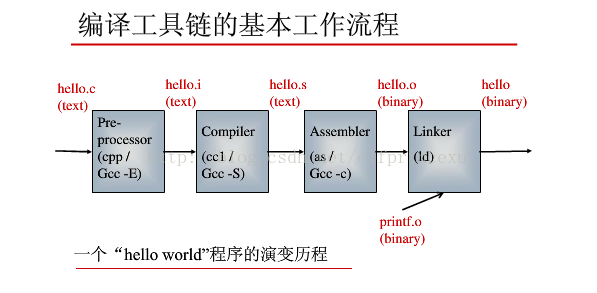
\includegraphics[width=4in]{slide01/images/compile.png}
    \caption{编译过程}
    \label{fig:1}
  \end{figure}
  
\end{frame}


\begin{frame}[fragile]\ft{\secname}
  执行以下命令,会在当前目录下生成所有的中间文件以及可执行文件。
  \begin{lstlisting}[backgroundcolor=\color{red!10}]
    $ gcc -Wall -save-temps hello.c –o hello 
    $ ls 
    hello     hello.c   hello.o
    hello.i   hello.s
  \end{lstlisting}
\end{frame}


\begin{frame}[fragile]\ft{\secname} 
  \begin{itemize}
  \item[(1)] \red{预处理阶段}
\begin{lstlisting}[backgroundcolor=\color{red!10}]
$ gcc -E hello.c –o hello.i 
\end{lstlisting}    
\end{itemize}

在该阶段,
    \begin{itemize}
    \item 去掉注释
    \item 宏的展开
    \item 头文件的展开
    \item 选项 \blue{\lstinline|-E|} 的作用是让gcc在预处理结束后停止编译过程。
    \end{itemize}   
\end{frame}


\begin{frame}[fragile]\ft{\secname}
  \begin{lstlisting}[basicstyle=\ttfamily\footnotesize,backgroundcolor=\color{red!10}]
    $ less hello.i
    $ ls 
    ...
    extern int printf (const char *__restrict __format, ...);
    ...
    # 868 "/usr/include/stdio.h" 3 4
    # 5 "hello.c" 2
    # 5 "hello.c"

    int main(void)
    {
      printf("Hello World!\n");
      return 0;
    }
  \end{lstlisting}
\end{frame}


% \begin{frame}[fragile]\ft{\secname}
%   \blue{分析:}在以上内容中,源文件被附加了很多信息,但在末尾代码仍被保留。{\ttfamily printf()}函数中包含了{\ttfamily a+b}而非{\ttfamily add(a,b)},因为宏已被展开。注释被去除掉。{\ttfamily\#include<stdio.h>}没有了,取而代之的是很多代码。因此,头文件已被展开,并且被包含到了源文件中。

% \end{frame}


\begin{frame}[fragile]\ft{\secname}
  \begin{itemize}
  \item[(2)] 编译阶段
\begin{lstlisting}[backgroundcolor=\color{red!10}]
$ gcc -S hello.i –o hello.s
\end{lstlisting}
\end{itemize}

在该阶段,
\begin{itemize}
\item 检查代码的规范性、是否有语法错误等
\item 检查无误后,将代码翻译成汇编语言
\item 选项 \blue{\lstinline|-S|} 只进行编译,不进行汇编,生成汇编代码。 
\end{itemize}

\end{frame}


\begin{frame}[fragile]\ft{\secname}
  \begin{lstlisting}[basicstyle=\ttfamily\footnotesize,backgroundcolor=\color{red!10}]
    $ less hello.s
    ...
    movl    $0, -4(%rbp)
    movl    $5, -8(%rbp)
    movl    $4, -12(%rbp)
    movl    -8(%rbp), %eax
    addl    -12(%rbp), %eax
    movl    %eax, %esi
    movb    $0, %al
    callq   _printf
    xorl    %esi, %esi
    ...      
  \end{lstlisting}
  % 以上内容表明这是汇编语言,能为汇编器所识别。
\end{frame}


\begin{frame}[fragile]\ft{\secname}
  \begin{itemize}
  \item[(3 )] 汇编阶段
\begin{lstlisting}[backgroundcolor=\color{red!10}]
$ gcc -c hello.s –o hello.o
\end{lstlisting}   
\end{itemize}

在该阶段,
\begin{itemize}
\item 将通过汇编器将 \lstinline|hello.s| 转换成  二进制机器指令文件\lstinline|hello.o|。
\item 只会将现有代码转换成机器语言,而诸如 \lstinline|printf()| 的函数调用则不会。
\item 选项 \blue{\lstinline|-c|} 的作用是将汇编代码转换为二进制目标代码。
\end{itemize}
\end{frame}


\begin{frame}[fragile]\ft{\secname}
  \begin{lstlisting}[backgroundcolor=\color{red!10}]
    $ less hello.o
    <CF><FA><ED><FE>^G^@^@^A^C^@^@^@^A^@^@^@^D^@^@^@^@^B^@^@^@ ^@^@^@^@^@^@^Y^@^@^@<88>^A^@^@^@^@^@^@^@^
    ...      
  \end{lstlisting}

\end{frame}


\begin{frame}[fragile]\ft{\secname}
  \begin{itemize}
  \item[(4)] 链接阶段
  \item[] 
    这里涉及一个重要的概念:\red{函数库}。 
  \end{itemize} \pause
  \begin{question}[]{}
    在 \lstinline|hello.c|中,并没有定义 \blue{\lstinline|printf()|} 的函数实现,并且在 \blue{\lstinline|stdio.h|} 也只有函数的声明,没有定义函数的实现。那么,是在哪里实现了 \blue{\lstinline|printf()|} 呢?
  \end{question} \pause

  事实上,系统将这些函数的定义编译后放在了相应的函数库中。在没有特别指定时,gcc 会到系统默认的搜索路径 \blue{\lstinline|/usr/lib|} 下进行查找,连接到相关的库函数后,就能使用 \blue{\lstinline|printf()|}了,而这就是链接的作用。
 
\end{frame}


% \begin{frame}[fragile]\ft{\secname}
%   在命令行中输入以下命令,可看出从目标文件到可执行文件时文件大小的变化。这是因为链接器为我们的程序添加了额外的代码。
%   \begin{lstlisting}[basicstyle=\ttfamily\footnotesize,backgroundcolor=\color{red!10}]
%     $ size hello.o
%     __TEXT  __DATA  __OBJC  others    dec         hex
%     145     0       0       32      177         b1        
%     $ size hello
%     __TEXT  __DATA  __OBJC  others    dec         hex
%     4096      4096    0  4294971392 4294979584 100003000
%   \end{lstlisting}

% \end{frame}


\begin{frame}{函数库}
  \href{http://www.cnblogs.com/skynet/p/3372855.html}{函数库}一般分为静态库和动态库。
  \begin{defn}[静态库]{}
    在链接阶段,将汇编生成的目标文件.o与引用到的库文件一起链接打包到可执行文件,对应的链接方式成为\red{静态链接}。
  \end{defn}

  \begin{defn}[动态库]{}
    \red{动态库}在程序编译时并不会被连接到目标代码中,而是在程序运行是才被载入。
  \end{defn}
\end{frame}

\begin{frame}{静态库}
  \begin{free}[静态库的特点]{}
    \begin{itemize}
    \item 一个静态库可以简单看成是一组目标文件(.o/.obj文件)的集合,即很多目标文件经过压缩打包后形成的一个文件。\\[.1in]
    \item 静态库对函数库的链接是放在编译时期完成的 \\[.1in]
    \item 程序在运行时与函数库再无瓜葛,移植方便 \\[.1in]
    \item 浪费空间与资源,因为所有相关的目标文件与牵涉到的函数库被链接合并成一个可执行文件\\[.1in]
    \item 后缀名为 \blue{\lstinline|.a|} (linux) 或 \blue{\lstinline|.lib|} (windows)
    \end{itemize}
  \end{free}

\end{frame}

\begin{frame}{静态库}
  \begin{figure}
    \centering
    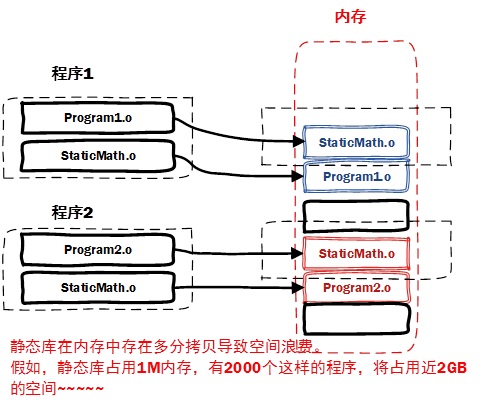
\includegraphics[width=3.5in]{slide01/images/lib.png}
    % \caption{静态库}
  \end{figure}
\end{frame}

\begin{frame}{静态库}
  \begin{free}[静态库的缺点]{}
    \begin{itemize}
    \item 空间浪费
    \item 静态库对程序的更新、部署和发布页会带来麻烦。如果静态库liba.lib更新了,所以使用它的应用程序都需要重新编译、发布给用户(对于玩家来说,可能是一个很小的改动,却导致整个程序重新下载,全量更新)。    
    \end{itemize}
  \end{free}
\end{frame}


\begin{frame}{动态库}
  \begin{free}[动态库的特点]{}
    \begin{itemize}
    \item 不同的应用程序如果调用相同的库,那么在内存里只需要有一份该共享库的实例,规避了空间浪费问题。 \\[.05in]
    \item 动态库在程序运行是才被载入,也解决了静态库对程序的更新、部署和发布页会带来麻烦。用户只需要更新动态库即可,增量更新。 \\[.05in]
    \item 后缀名为 \blue{\lstinline|.so|} (linux) 或 \blue{\lstinline|.dll|} (windows) \\[0.05in]
    \item gcc 在编译时默认使用动态库
    \end{itemize}
  \end{free}

\end{frame}


\begin{frame}{动态库}
  \begin{figure}
    \centering
    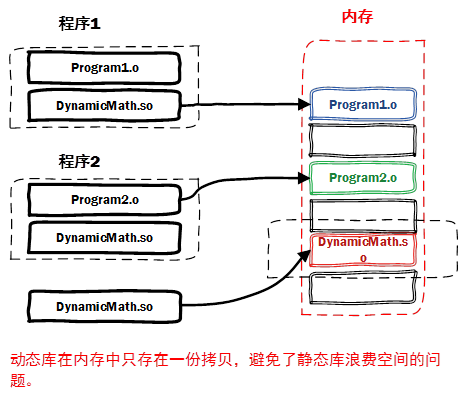
\includegraphics[width=3.5in]{slide01/images/dll.png}
    %\caption{动态库}
  \end{figure}
\end{frame}

\begin{frame}{函数库的创建与使用}
  设有4个文件:
  \begin{itemize}
  \item \lstinline|hello.h|
  \item \lstinline|hello1.c|
  \item \lstinline|hello2.c|
  \item \lstinline|main.c|
  \end{itemize}
  我们来看看如何创建静态库与动态库,并如何使用它们。
\end{frame}

\begin{frame}{函数库的创建与使用}
  \lstinputlisting[title=hello.h]{slide01/code/lib/hello.h}
\end{frame}

\begin{frame}{函数库的创建与使用}
  \lstinputlisting[title=hello1.c]{slide01/code/lib/hello1.c}

  \lstinputlisting[title=hello2.c]{slide01/code/lib/hello2.c}
\end{frame}

\begin{frame}{函数库的创建与使用}
  \lstinputlisting[title=main.c]{slide01/code/lib/main.c}
\end{frame}

\begin{frame}[fragile]{静态库的创建与使用}

  \begin{lstlisting}
# 将 hello.c 编译成 hello.o (静态库和动态库都由 .o 文件生成)
$ gcc -c hello1.c hello2.c

# 为遵循 linux 中静态库的命名规范,静态库命名为 libhello.a
$ ar -crv libhello.a hello1.o hello2.o

# 将 main.c 与静态库连接,生成可执行文件 main
$ gcc main.c -L. -lhello -o main

# 运行 main
$ ./main
  \end{lstlisting}
  
\end{frame}


\begin{frame}[fragile]{动态库的创建与使用}

  \begin{lstlisting}
# 将 hello.c 编译成一个动态库 libhello.so
$ gcc hello1.c hello2.c -fPIC -shared -o libhello.so

# 将 main.c 与动态库连接,生成可执行文件 main
$ gcc main.c -L. -lhello -o main 

# 运行 main
$ ./main
  \end{lstlisting}
  
\end{frame}


